\chapter{Object Selection}\label{cha:object_selection}

\section{Tracks and Vertices}\label{sec:object_selection:tracks_and_vertices}

\section{Electrons}\label{sec:object_selection:electrons}

Electrons can be identified with a high precision and large background rejection by matching clusters of energy
depositions in the electromagnetic calorimeter with extrapolations of reconstructed tracks provided by the ID\@.
Because of the good performance of the electromagnetic calorimeter and inner detector their energy and momentum can
be determined with a good precision.
To suppress background contributions from pile-up events or other objects like jets and hadronically decaying $\tau$-leptons
additional information of the ID and hadronic calorimeter are considered.

The identification algorithm~\cite{ATLAS-CONF-2016-024} is a likelihood-based method, which uses a multivariate analysis (MVA) technique to
evaluate multiple properties of the electron candidate.
Different requirements on the likelihood discriminant\footnote{The discriminant is defined as
$\frac{\mathcal{L}_S}{\mathcal{L}_S + \mathcal{L}_B}$, where $\mathcal{L}_S$ and $\mathcal{L}_B$ denote the product of
the signal and background probability density functions of the used variables.} yield different operating points,
labeled as  \emph{loose}, \emph{medium}, and \emph{tight}.
They provide a different level of electron identification efficiency and background rejection.

In this analysis the \emph{loose} criterion is chosen.
Additional requirements are $\pt > \unit[15]{GeV}$ and $\abs{\eta} < 2.47$.
The Pixel Detector and SCT can only provide information for reconstruction and identification in this $\eta$-range.
Electrons within $1.37 < \abs{\eta} < 1.52$ are excluded, because of the poor reconstruction and identification
performance caused by the crack between the barrel and end-calorimeters.

To increase the background rejection, isolation requirements are introduced by the following two discriminating variables.
The calorimetric isolation energy $\et^{\text{cone}0.2}$ is defined as the sum of transverse energy deposited within
$\dr = 0.2$ around the electron candidates.
Corrections for electron energy leakage, pile-up, and the underlying event activity are applied.
The sum of the transverse momentum of all tracks within $\dr = \min(0.2, \unit[10]{GeV} / \et)$ builds the
track isolation $\pt^{\text{varcone}0.2}$. The tracks need to fulfill certain quality requirements and have to originate
from the primary vertex.
Based on different selections criteria on quantities $\et^{\text{cone}0.2} / \et$ and
$\pt^{\text{varcone}0.2} / \et$ multiple operating points are constructed. This analysis uses the \emph{gradient}
isolation criterion with a targeted efficiency of
$\unit[0.1143]{\%} \times \et / \text{GeV} + \unit[92.14]{\%}$~\cite{ATLAS-CONF-2016-024}.

The efficiencies of the electron identification and isolation criteria are measured using a \emph{tag-and-probe technique}
in $\Z \to \epem$ and $\JPsi \to \epem$ events.
The \emph{tag} electron must pass the \emph{tight} identification criterion as well as some other selection criteria.
Because of the chosen events it is very probable that a second electron, the \emph{probe}, is contained in this event.
By counting how many \emph{probe} electrons pass the different identification and isolation requirements the efficiencies
of those working points can be obtained.
The combined reconstruction and identification efficiencies in $\Z \to \epem$ events as a function of $\et$ and $\eta$
are shown in \cref{fig:object_selection:el_id_eff}.
In account to correct for differences in data and simulated events the efficiencies are calculated for both event types.
The ratio is then used to derive \emph{scale factors}, which are applied to the simulated events in this analysis.

% TODO energy resolution ?

\begin{figure}[htb]
    \begin{center}
        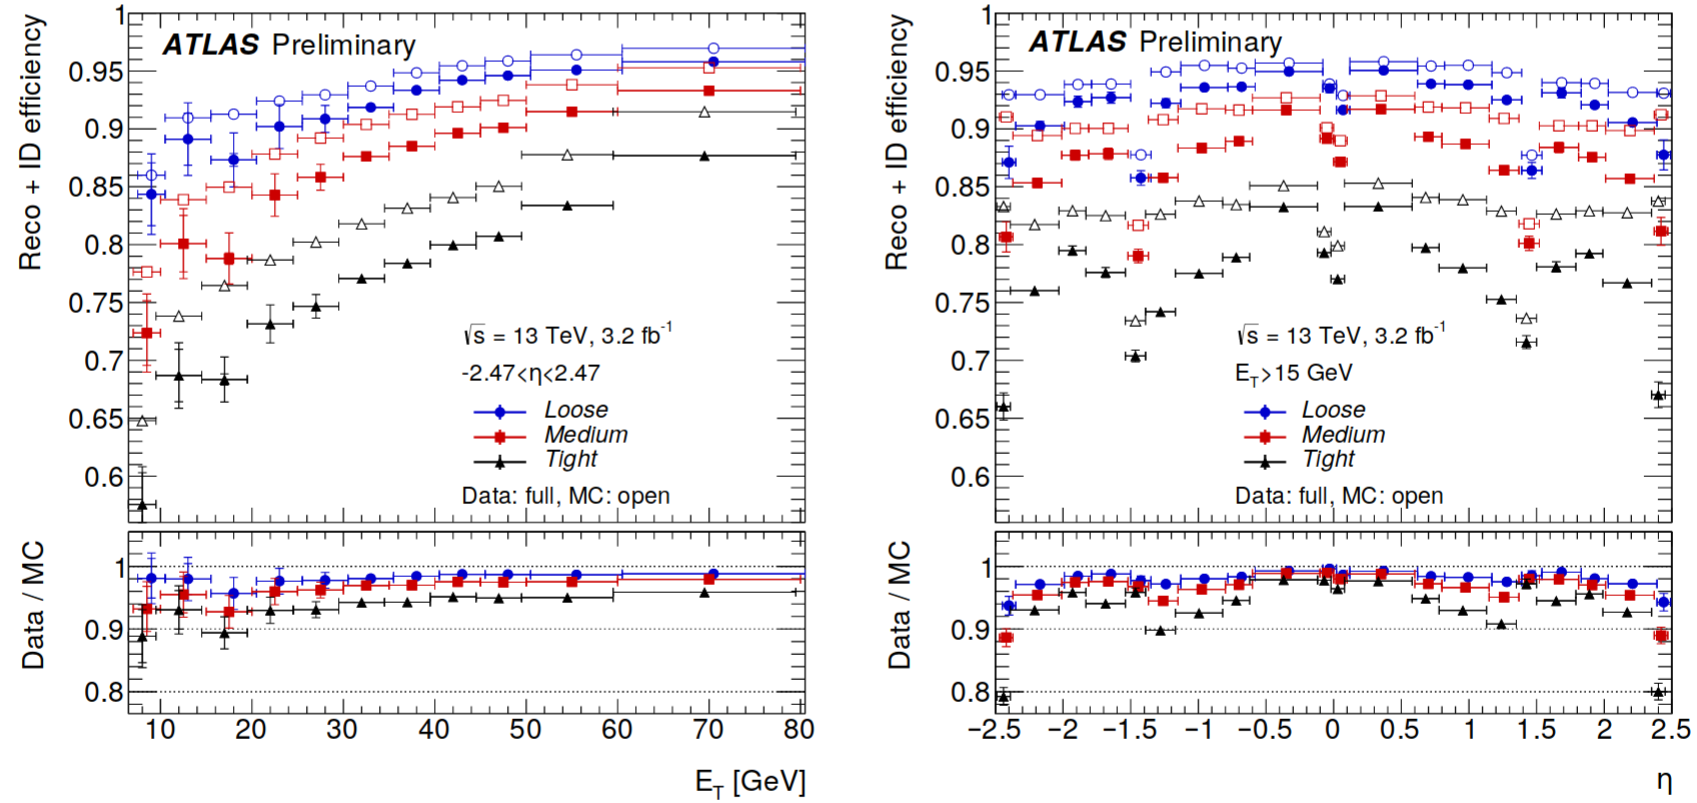
\includegraphics[width=0.9\textwidth]{./figures/object_selection/el_id_eff.png}
        \caption{Combined electron reconstruction and identification efficiencies for $\Z \to \epem$ events as a
                 function of $\et$ (left) and $\eta$ (right) for the \emph{loose}, \emph{medium}, and \emph{tight}
                 working points. The inner error bars show the statistical uncertainty, the outer error bars combine
                 the statistical and systematic uncertainties.~\cite{ATLAS-CONF-2016-024}}\label{fig:object_selection:el_id_eff}
    \end{center}
\end{figure}

\section{Muons}\label{sec:object_selection:muons}

Muons are reconstructed by taking into account information of the inner detector (ID), calorimeter, and the
muon spectrometer (MS).
Because  they traverse the detectors with minimum energy loss, they have a clear signature in the detectors and the
discrimination between them and other physics objects like electrons and jets reaches a high accuracy.

First, muons are reconstructed independently in the ID and the MS\@. The track reconstruction in the ID follows the
usual prescriptions for charged particles~\cite{ATL-SOFT-PUB-2007-007,ATLAS-CONF-2010-072}.
For the track reconstruction in the MS each muon chamber is searched for hit patterns, which are combined to track
segments. The segments are then combined to muon track candidates. For each track candidate a global $\chi^2$ fit
is performed to the hits associated with the track. If a certain threshold is reached the track is accepted~\cite{PERF-2015-10}.

After the individual reconstruction four different algorithms are applied to combine the information of the different
sub-detector systems.
Combined (CB) muons have both a track in the ID and MS\@. The global track is calculated by a refit to both tracks.
If there is only one local track segment in the MDT or CSC chambers and the track of the ID can be extrapolated to the MS
the muon is classified as segment-tagged (ST).
A track in the ID can be classified as calorimeter-tagged (CT) muon if the track can be matched to a energy deposition
in the calorimeter, if it has the signature of a minimum-ionizing particle.
Extrapolated (ME) muons are reconstructed only from tracks in the MS with the additional requirement that the track
needs to originate from the interaction point (IP)\@.

To reduce background from mainly pion and kaon decays, different muon identification criteria are defined.
For \emph{medium} muons only CB and ME tracks are used with some additional requirements on the number of hits in
different layers and the \emph{q/p significance}\footnote{The \emph{q/p significance} is the absolute value of the
difference between charge and momentum measured in ID and MS divided by the sum of squares of the respective uncertainties.}.
In this analysis \emph{loose} muons are used with $\pt > \unit[10]{GeV}$ and $\abs{\eta} < 2.5$.
This includes all \emph{medium} muons as well as CT and ST muons, which are however restricted to $\abs{\eta} < 0.1$.

Isolation requirements can further reduce background, because muons originating from heavy particles like $\W$, $\Z$,
or Higgs bosons are often produced isolated. Two discriminating variables are introduced.
The calorimetric isolation energy $\et^{\text{topocone}20}$ is defined as the sum of transverse energy deposited within
$\dr = 0.2$ around the muon candidates.
Corrections for pile-up and the underlying event activity are applied.
The sum of the transverse momentum of all tracks with $\pt > \unit[1]{GeV}$ within $\dr = \min(0.3, \unit[10]{GeV} / \pt^\mu)$
is defined as the track isolation $\pt^{\text{varcone}0.3}$.
Based on different selections criteria on quantities $\et^{\text{topocone}20} / \pt^\mu$ and
$\pt^{\text{varcone}30} / \pt^\mu$ multiple operating points are constructed.
This analysis uses the \emph{gradient} isolation criterion which provides an efficiency of more than
$\unit[90(99)]{\%}$ at $\unit[20(60)]{GeV}$~\cite{PERF-2015-10}.

The muon reconstruction and identification efficiencies are obtained with a \emph{tag-and-probe technique} using
$\Z \to \mpmm$ and $\JPsi \to \mpmm$ events.
\cref{fig:object_selection:mu_id_eff} shows the reconstruction efficiencies for \emph{medium} and \emph{loose} muons.
The efficiencies are calculated both in data and simulated events in order to derive \emph{scale factors}, which are used
to correct deviations of the efficiencies in data and simulation.

\begin{figure}[htb] % TODO fix vertical label position
    \begin{center}
        \begin{subfigure}[c]{0.45\textwidth}
            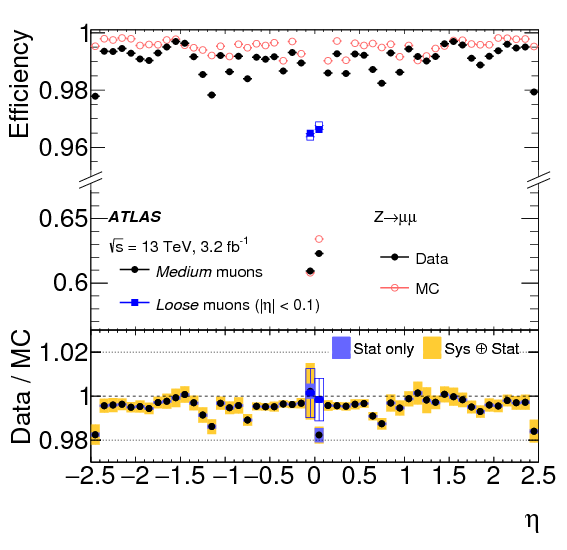
\includegraphics[width=\textwidth]{./figures/object_selection/mu_id_eff_a.png}
            \caption{}
        \end{subfigure}
        \hfill
        \begin{subfigure}[c]{0.45\textwidth}
            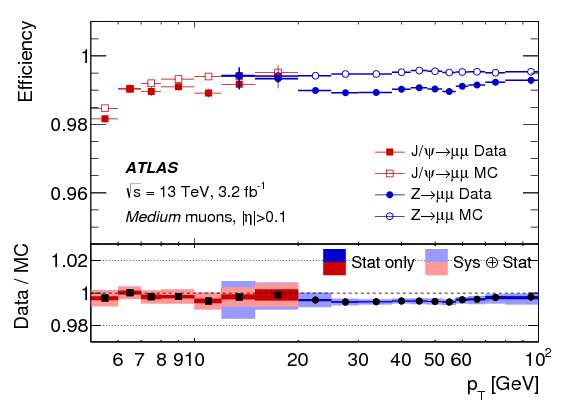
\includegraphics[width=\textwidth]{./figures/object_selection/mu_id_eff_b.png}
            \caption{}
        \end{subfigure}
        \caption{Muon reconstruction efficiencies for \emph{loose} and \emph{medium} muons as a function of $\eta$
                measured in $\Z \to \mpmm$ events (a) and for \emph{medium} muons as a function of $\pt$ measured in
                $\Z \to \mpmm$ and $\JPsi \to \mpmm$ events (b).~\cite{PERF-2015-10}}\label{fig:object_selection:mu_id_eff}
    \end{center}
\end{figure}


\section{Jets}\label{sec:object_selection:jets}

\section{Tau Leptons}\label{sec:object_selection:tau_leptons}

\section{Missing Transverse Energy}\label{sec:object_selection:missing_transverse_energy}

\section{Overlap Removal}\label{sec:object_selection:overlap_removal}


